\documentclass[10pt]{article}

% DOCUMENT LAYOUT
%\usepackage{fullpage}
%\usepackage[cm]{fullpage}
%\usepackage[letterpaper, top=0.5in, bottom=0.5in, left=0.5in, right=0.5in]{geometry} 
%\usepackage[letterpaper]{geometry} 
%\geometry{textwidth=5.7in, textheight=9.0in, marginparsep=7pt, marginparwidth=.6in}
%\geometry{textwidth=6.0in, textheight=9.8in, marginparsep=7pt, marginparwidth=.8in}
%\geometry{textwidth=6in, textheight=9.8in, marginparsep=7pt, marginparwidth=.8in}
\setlength\parindent{0in}

%\addtolength{\oddsidemargin}{-.500in}
%\addtolength{\evensidemargin}{-.500in}
%\addtolength{\textwidth}{2.00in}
\addtolength{\topmargin}{-.875in}
\addtolength{\textheight}{1.75in}

\addtolength{\oddsidemargin}{-.375in}
\addtolength{\evensidemargin}{-.375in}
\addtolength{\textwidth}{1.75in}
\addtolength{\marginparsep}{-10pt}
\addtolength{\marginparwidth}{+15pt}

\usepackage{wrapfig}

\usepackage{chngpage}
\usepackage[export]{adjustbox}

% SPECIAL FORMATTING
% ---- CUSTOM AMPERSAND
\newcommand{\amper}{{\selectfont\itshape\&}}
% ---- MARGIN YEARS
%\newcommand{\years}[1]{\marginpar{\scriptsize #1}}
\newcommand{\years}[1]{\marginpar{\quad \small #1}}
% ---- TALK COUNTER
\newcounter{talknumber}
\setcounter{talknumber}{1}
% ---- ARTICLE COUNTER
\newcounter{articlenumber}
\setcounter{articlenumber}{1}
%\newcommand{\article}{\noindent\marginpar{\scriptsize \arabic{articlenumber}}\addtocounter{articlenumber}{1}}
\newcommand{\article}[2]{
\noindent\marginpar{
  \parbox[c]{0.25in}{\scriptsize \arabic{articlenumber}} 
  \parbox[c]{0.25in}{\scriptsize \href{#2}{#1}}
}\addtocounter{articlenumber}{1}}
% PAPER DESCRIPTION AND THUMBNAIL IMAGE
\newcommand{\desc}[2]{
\noindent\marginpar{
  \parbox[c]{0.50in}{{\includegraphics[width=0.9in]{thumbnails/{#1}}}}
}{\footnotesize\emph{#2}}}
% NEW ARTICLE STYLE WITH IMAGE AND NO NUMBERS
\newcommand{\newarticle}[5]{
\begin{adjustwidth}{-1in}{-1in}  
\begin{tabular}{p{0.9in}p{7in}}
\parbox[c]{0.9in}{\includegraphics[width=0.9in]{thumbnails/{#1}}} & \parbox[c]{6in}{{#2} $\cdot$ \href{#4}{#3} \\ {\footnotesize\emph {#5}}}
\end{tabular}
\end{adjustwidth}
\vspace{0.2in}
}

% ---- TALKS
\newcommand{\talk}[2]{
\noindent\marginpar{
   \scriptsize \scshape
  #2 \\ #1
}}
\newcommand{\numberedtalk}[2]{
\noindent\marginpar{
  \parbox[c]{0.25in}{\scriptsize \arabic{talknumber}} 
% \parbox[c]{0.5in}{\scriptsize {#2}}
  \parbox[c]{0.5in}{\scriptsize \scshape {#1}}
}\addtocounter{talknumber}{1}}

\newcommand{\newtalk}[3]{
\noindent\marginpar{
   \scriptsize \scshape
  #2 \\ #1
}\spaceTalk\\}

% SPACING
\newcommand{\spaceEd}{\vspace{1ex}}
\newcommand{\spaceRes}{\vspace{1ex}}
\newcommand{\spaceFell}{\vspace{0.5ex}}
\newcommand{\spacePub}{\vspace{0.5ex}}
\newcommand{\spaceTalk}{\vspace{1ex}}
\newcommand{\spaceSoc}{\vspace{0.5ex}}
\newcommand{\spacePost}{\vspace{0.5ex}}

% GRAPHICS
\usepackage{graphicx}

% HEADINGS
\usepackage{sectsty} 
\usepackage[normalem]{ulem} 

\usepackage{fancyhdr}
\pagestyle{fancy}
\fancyhf{}
\rfoot{\small\textsc{John D. Chodera - Curriculum Vitae - \thepage}}

% Clean up font spacing with micro type
\usepackage{microtype}

% Use a clean, modern-looking font
\usepackage[default]{lato}
\usepackage[T1]{fontenc}

% Change the appearance of section and subsection headings
\sectionfont{\mdseries\large\underline} 
\subsectionfont{\mdseries\scshape\normalsize} 
\subsubsectionfont{\bfseries\upshape\normalsize} 

% Control tightness of spacing
\renewcommand{\baselinestretch}{1.1}

% PDF SETUP
% ---- FILL IN HERE THE DOC TITLE AND AUTHOR
\usepackage[bookmarks, colorlinks, breaklinks, pdftitle={John D. Chodera - vita},pdfauthor={John D. Chodera}]{hyperref}  
\hypersetup{linkcolor=blue,citecolor=blue,filecolor=black,urlcolor=blue} 

% Change the typewriter font to something nicer.
\usepackage[ttdefault]{sourcecodepro}

% DOCUMENT
\begin{document}
\reversemarginpar
% FILL IN NAME HERE
{\fontseries{eb}\selectfont \LARGE John D. Chodera}\\[1cm]

% FILL IN AUTHOR INFORMATION HERE
\begin{minipage}[t]{2.5in}
%
\includegraphics[width=0.7in,valign=c]{images/john_chodera_sm.pdf}
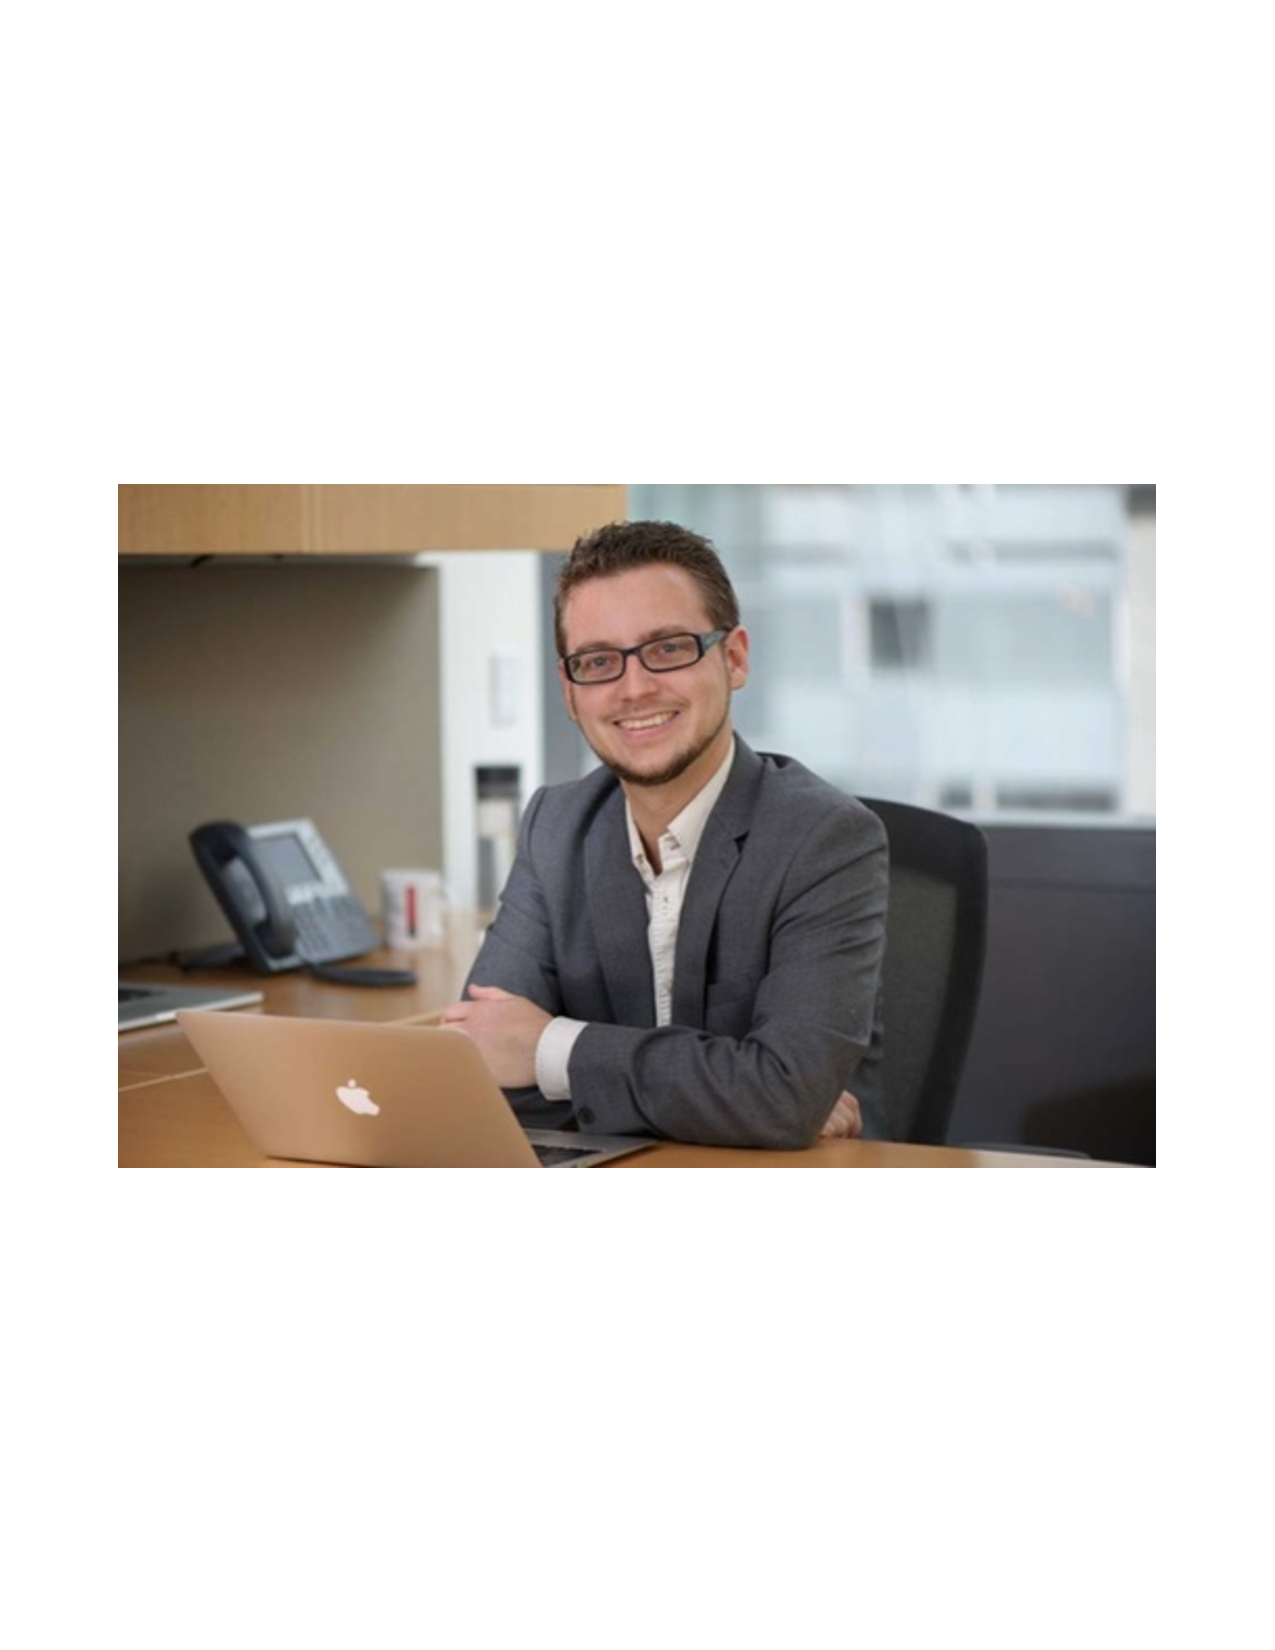
\includegraphics[width=2.5in,valign=c]{images/john_chodera_wide.pdf}
\end{minipage}
\quad
\begin{minipage}[t]{3in}
\begin{tabular}{rl}
{\bf email} & \href{mailto:choderaj@mskcc.org}{\href{mailto:john.chodera@choderalab.org}{john.chodera@choderalab.org}}\\
{\bf url} & \href{http://www.choderalab.org}{\href{http://www.choderalab.org}{http://www.choderalab.org}}\\[0.05in]
{\bf tel} & 646.888.3400\\[0.05in]
{\bf fax} & 510.280.3760 \\[0.05in]
{\bf mobile} & 646.737.3319\\[0.05in]
{\bf post} & 
\parbox[t]{3.0in}{Memorial Sloan-Kettering Cancer Center\\
1275 York Ave, Box 357\\
New York, NY 10065}
\end{tabular}
\end{minipage}

% RESEARCH INTERESTS
%\section*{Research interests}
%\noindent {\bf Computational biophysics}, especially \\
%\noindent {\bf Single-molecule biophysics}, including new techniques for interpreting force microscopy \\
%\noindent {\bf Nonequilibrium statistical mechanics}, as tools for single-molecule experimental probes and the design of new algorithms for computational chemistry \\

\section*{Education and positions}

\noindent\years{2013--}{\bf Assistant Professor, Physiology, Biophysics, and Systems Biology Program,\\
Weill Cornell Graduate School of Medical Sciences}\\
\noindent\years{2012--}{\bf Assistant Member, Memorial Sloan-Kettering Cancer Center}\\
\noindent\years{2008--2012}{\bf Independent Distinguished Postdoctoral Fellow, California Institute for Quantitative Biosciences (QB3),\\
University of California, Berkeley}\\
Independent research funding, sponsors \href{http://chem.berkeley.edu/faculty/geissler/index.php}{Phillip L. Geissler} and \href{http://zebra.berkeley.edu/}{Susan Marqusee} \\
%\noindent\years{2011--2012}{\bf \href{http://research.google.com/university/exacycle_program.html}{Google Exacycle Visiting Faculty}} \\
\noindent\years{2006--2008}{\bf Postdoctoral researcher, Department of Chemistry, Stanford University}\\
With \href{http://folding.stanford.edu/Pande/Main}{Vijay S. Pande} (head of \href{http://folding.stanford.edu}{Folding@Home} distributed computing project) \\
\noindent\years{1999--2006}{\bf \textsc{Ph.D.} in Biophysics, University of California, San Francisco}\\
%Dissertation: \href{http://www.dillgroup.ucsf.edu/~jchodera/pubs/pdf/jdcthesis.pdf}{\emph{Master equation models of macromolecular dynamics from atomistic simulation.}} \\
Committee: \href{http://www.dillgroup.org}{Ken A. Dill}, \href{http://jacobsonlab.org/}{Matthew P. Jacobson}, \href{http://folding.stanford.edu/Pande/Main}{Vijay S. Pande}\\
\noindent\years{1995--1999}{\bf \textsc{B.S.} in Biology, California Institute of Technology}\\
Undergraduate research with \href{http://www.its.caltech.edu/~phplab/phplab.html}{Paul H.~Patterson} (\emph{experimental molecular neurobiology}) \\and Jerry E.~Solomon (\emph{computational chemistry}).

\section*{Fellowships and awards}

\noindent\years{2013--2016}Louis V.~Gerstner Young Investigator Award\\
\noindent\years{2013--2014}Google Exacycle for External Faculty\\
\noindent\years{2008--2012}QB3-Berkeley Distinguished Postdoctoral Fellowship, University of California, Berkeley\\
%\noindent\years{2008}Berkeley Mini Stat Mech Meeting Best Poster Prize (second place)\\
\noindent\years{2005--2006}IBM Predoctoral Fellowship\\
\noindent\years{2005}Frank M. Goyan Award for outstanding work in physical chemistry, University of California, San Francisco\\
\noindent\years{2000--2005}Howard Hughes Medical Institute Predoctoral Fellowship\\
\noindent\years{1998--1999}Caltech Upperclass Merit Award Scholarship\\
\noindent\years{1997,$\:$1998}Caltech Summer Undergraduate Research Fellowships

\section*{Research interests}

\noindent{Rational computational drug design of small-molecule t 	herapeutics}\\
\noindent{Kinase inhibitor selectivity and evolution of therapeutic resistance in cancer}\\
\noindent{Multiscale modeling of the effects of small molecules on biochemical pathways}\\
\noindent{Biomolecular dynamics and conformational heterogeneity, allosteric inhibitor design}\\
\noindent{Error and uncertainty in biophysical measurements}\\
\noindent{Computational chemistry, molecular modeling, and forcefield development}

\eject

\section*{Publications}

Google Scholar statistics: \href{http://goo.gl/qO0JW}{http://goo.gl/qO0JW}\\

{\small \it h-index: 28 / i10-index: 41 / published or in press: 44}

{\scriptsize $^*$ asterisks denote that marked authors contributed equally}\\
{\scriptsize $^\dag$ daggers denote corresponding-author publication}

%%%%%%

\subsection*{Rational drug design}

\newarticle{identifying-ligand-binding-sites.pdf}{Wang K, {\bf Chodera JD}, Yang Y, and Shirts MR. Identifying ligand binding sites and poses using GPU-accelerated Hamiltonian replica exchange molecular dynamics. {\it J.~Comput.~Aid.~Mol.~Des.}, 27:989--1007, 2013.}{DOI}{http://dx.doi.org/10.1007/s10822-013-9689-8}{We show how bound ligand poses can be identified even when the location of the binding sites are unknown using the machinery of alchemical modern free energy calculations on graphics processors.}

\newarticle{entropy-enthalpy-compensation.pdf}{{\bf Chodera JD}$^\dag$ and Mobley DL. Entropy-enthalpy compensation: Role and ramifications for rational ligand design. {\it Annu.~Rev.~Biophys.}, 42:121, 2013}{DOI}{http://dx.doi.org/10.1146/annurev-biophys-083012-130318}{Entropy-enthalpy compensation is likely a universal phenomena, but not as severe as widely thought, and likely not of enormous concern for drug discovery and ligand design.}

\newarticle{alchemical-methods.pdf}{{\bf Chodera JD}, Mobley DL, Shirts MR, Dixon RW, Branson KM, and Pande VS. Free energy methods in drug discovery and design: Progress and challenges. {\it Curr.~Opin.~Struct.~Biol.}, 21:150--160, 2011}{DOI}{http://dx.doi.org/10.1016/j.sbi.2011.01.011}{A review of the opportunities and challenges for alchemical free energy calculations in drug discovery and design.}

\newarticle{mbar-equation.pdf}{Shirts MR, {\bf Chodera JD}. Statistically optimal analysis of samples from multiple equilibrium states. {\it J.~Chem.~Phys.} 129:124105, 2008}{DOI}{http://dx.doi.org/10.1063/1.2978177}{We present a highly general, statistically optimal approach for producing estimates of free energies and equilibrium expectations from multiple simulations that provably extracts all useful information from the data.}

\newarticle{small-molecule-solvation.pdf}{Nicholls A*, Mobley DL*, Guthrie JP, {\bf Chodera JD}, and Pande VS. Predicting small-molecule solvation free energies: A blind challenge test for computational chemistry. {\it J.~Med.~Chem.} 51:769--779, 2008}{DOI}{http://dx.doi.org/10.1021/jm070549+}{A blind evaluation of the accuracy of alchemical free energy methods for computing gas-to-water transfer free energies (solvation free energies) of small molecules demonstrates that modern forcefields are likely sufficiently accurate to be useful in drug design.}

\newarticle{entropy-solvation.pdf}{Mobley DL, Dill KA, and {\bf Chodera JD}. Treating entropy and conformational changes in implicit solvent simulations of small molecules. {\it J.~Phys.~Chem.~B} 112(3):938--946, 2008}{DOI}{http://dx.doi.org/10.1021/jp0764384}{An quantitative examination of how much conformational entropy contributes to hydration free energies of small molecules, with implications for ligand binding.}

\newarticle{long-range-dispersion-correction.pdf}{Shirts MR*, Mobley DL*, {\bf Chodera JD}, and Pande VS. Accurate and efficient corrections for missing dispersion interactions in molecular simulations.  {\it J.~Phys.~Chem.~B} 111(45):13052--13063, 2007}{DOI}{http://dx.doi.org/10.1021/jp0735987}{We identify a major source of systematic error in absolute alchemical free energy calculations of ligand binding and show how a simple procedure can inexpensively and accurately eliminate it.}

\newarticle{charge-models.pdf}{Mobley DL, Dumont E, {\bf Chodera JD}, Bayly CI, Cooper MD, and Dill KA. Comparison of charge models for fixed-charge force fields: Small-molecule hydration free energies in explicit solvent.  \emph{J.~Phys.~Chem.~B} 111:2242--2254, 2007}{DOI}{http://dx.doi.org/10.1021/jp0667442}{We compare a number of popular methods for deriving charge models for small molecules, deriving lessons about best practices for accurate simulations.}

\newarticle{binding-free-energy.pdf}{Shirts MR, Mobley DL, {\bf Chodera JD}. Alchemical free energy calculations: Ready for prime time? {\it Ann.~Rep.~Comput.~Chem.} 3:41--59, 2007}{DOI}{http://dx.doi.org/10.1016/S1574-1400(07)03004-6}{A review of current alchemical free energy methodologies assessing whether they are ready for practical use in drug discovery and ligand design.}

\newarticle{t4-lysozyme-l99a.pdf}{Mobley DL, Graves AP, {\bf Chodera JD}, McReynolds AC, Shoichet BK, and Dill KA. Predicting absolute ligand binding free energies to a simple model site. {\it J.~Mol.~Biol.} 371(4):1118--1134, 2007}{DOI}{http://dx.doi.org/10.1016/j.jmb.2007.06.002}{We show how alchemical free energy calculations are capable of accurate blind prediction of small-molecule binding affinities to a simple model protein binding site.}

\newarticle{t4-lysozyme-val111}{Mobley DL, {\bf Chodera JD}, and Dill KA. Confine-and-release method: Obtaining correct binding free energies in the presence of protein conformational change. {\it J.~Chem.~Theor.~Comput.} 3(4):1231--1235, 2007}{DOI}{http://dx.doi.org/10.1021/ct700032n}{We present a general scheme for obtaining correct ligand binding affinities when protein conformational change is implicated in ligand binding.}

\newarticle{orientational-restraints.pdf}{Mobley DL, {\bf Chodera JD}, and Dill KA. On the use of orientational restraints and symmetry corrections in alchemical free energy calculations. {\it J.~Chem.~Phys.} 125:084902, 2006}{DOI}{http://dx.doi.org/10.1063/1.2221683}{We illustrate how orientational restraints can be used to greatly reduce the computational effort in alchemical calculations of ligand binding free energies, and clarify how symmetry corrections are necessary when molecules contain symmetric or pseudosymmetric substituents.}

%%%%%%%%%%%%%%%%%%

\subsection*{Analytical biochemistry}

\newarticle{itc-enthalpogram.pdf}{Tellinghuisen JT and {\bf Chodera JD}. Systematic errors in isothermal titration calorimetry: Concentrations and baselines. {\it Anal.~Biochem.}, 414:297--299, 2011}{DOI}{http://dx.doi.org/10.1016/j.ab.2011.03.024}{A word of caution about large errors in isothermal titration calorimetry measurements arising from ligand concentration errors.}

%%%%%%%%%%%%%%%%%%

\subsection*{Molecular simulation theory and algorithms}

\newarticle{thermoml-benchmark.pdf}{Beauchamp KA, Behr JM, Rustenburg AS, Bayly CI, Kroenlein K, and {\bf Chodera JD}$^\dag$. Towards automated benchmarking of atomistic forcefields: Neat liquid densities and static dielectric constants from the {ThermoML} data archive.}{ar$\chi$iv}{https://github.com/choderalab/LiquidBenchmark/raw/master/manuscript/benchmark.pdf}{Molecular mechanics forcefields are critical to computed-guide drug design, but the benchmarking and improvement of these forcefields has been hindered by the lack of high-quality machine-readable physical property datasets. We show how the NIST-curated ThemoML dataset, which stores physical property data in an IUPAC-standard format, can eliminate these roadblocks and reveal issues with current generation forcefields.}

\newarticle{ensembler.pdf}{Parton DL, Grinaway PB, Hanson SM, Beauchamp KA, and {\bf Chodera JD}. Ensembler: Enabling high-throughput molecular simulations at the superfamily scale.}{bioR$\chi$v}{http://dx.doi.org/10.1101/018036}{We demonstrate a new tool that enables---for the first time---massively parallel molecular simulation studies of biomolecular dynamics at the superfamily scale, illustrating its application to protein tyrosine kinases, an important class of drug targets in cancer.}

\newarticle{timestep-rescaling.pdf}{Sivak DA, {\bf Chodera JD}, and Crooks GE. Time step rescaling recovers continuous-time dynamical properties for discrete-time Langevin integration of nonequilibrium systems. {\it J. Phys. Chem. B}, 118:6466--6474, 2014.  William C.~Swope Festschrift.}{DOI}{http://dx.doi.org/10.1021/jp411770f}{We derive a simple, easy-to-implement Langevin integrator that has universally useful properties in molecular simulations.}

\newarticle{iamoeba-water}{Wang L-P, Head-Gordon TL, Ponder JW, Ren P, {\bf Chodera JD}, Eastman PK, Martinez TJ, and Pande VS. Systematic improvement of a classical molecular model of water. {\it J.~Phys.~Chem.~B}, 117:9956--9972, 2013}{DOI}{http://dx.doi.org/10.1021/jp403802c}{A new inexpensive polarizable model of liquid water for next-generation forcefields is derived using an automated parameterization engine.}

\newarticle{nonequilibrium-fluctuation-theorems}{Sivak DA, {\bf Chodera JD}, and Crooks GE. Using nonequilibrium fluctuation theorems to understand and correct errors in equilibrium and nonequilibrium discrete Langevin dynamics simulations. {\it Phys.~Rev.~X.}, 3:011007, 2013}{DOI}{http://dx.doi.org/10.1103/PhysRevX.3.011007}{The finite-timestep errors in molecular dynamics simulations can be interpreted as a form of nonequilibrium work.  We show how this leads to straightforward schemes for correcting for these errors or assessing their impact.}

\newarticle{gibbs-sampling.pdf}{{\bf Chodera JD} and Shirts MR. Replica exchange and expanded ensemble simulations as Gibbs sampling: Simple improvements for enhanced mixing. \emph{J.~Chem.~Phys.}, 135:194110, 2011}{DOI}{http://dx.doi.org/10.1063/1.3660669}{We show how a simple change to the way exchanges are handled in the popular replica-exchange simulation methodology can enormously increase efficiency at no increase in computational cost.}

\newarticle{ncmc.pdf}{Nilmeier JP, Crooks GE, Minh DDL, and {\bf Chodera JD}$^\dag$. Nonequilibrium candidate Monte Carlo is an efficient tool for equilibrium simulation. {\it Proc.~Natl.~Acad.~Sci.~USA.}, 108:E1009, 2011}{DOI}{http://dx.doi.org/10.1073/pnas.1106094108}{We present a significant generalization of Monte Carlo methods that provide an enormously useful tool for enhancing the efficiency of molecular simulations and enabling molecular design.}

\newarticle{current-status-amoeba.pdf}{Ponder JW, Wu C, Ren P, Pande VS, {\bf Chodera JD}, Mobley DL, Schnieders MJ, Haque I, Lambrecht DS, DiStasio RA Jr., Head-Gordon M,  Clark GNI, Johnson ME, and Head-Gordon T. Current status of the AMOEBA polarizable force field. {\it J.~Phys.~Chem.~B} 114:2549, 2010}{DOI}{http://dx.doi.org/10.1021/jp910674d}{A report on the status of the AMOEBA polarizable force field and its ability to reproduce a diverse set of physical chemical phenomenon to high accuracy.}

\newarticle{alanine-dipeptide-2dpmf.pdf}{{\bf Chodera JD}, W. C. Swope, J. W. Pitera, C. Seok, and K. A. Dill. Use of the weighted histogram analysis method for the analysis of simulated and parallel tempering simulations. \emph{J.~Chem.~Theor.~Comput.} 3(1):26--41, 2007}{DOI}{http://dx.doi.org/10.1021/ct0502864}{The weighted histogram analysis method (WHAM), a mainstay of molecular dynamics simulation analysis, is thoroughly explained and modernized for the analysis of simulated and parallel tempering simulation data.}

\newarticle{moped.pdf}{Seok C, Rosen JB, {\bf Chodera JD}, Dill KA. MOPED: Method for optimizing physical energy parameters using decoys. {\it J.~Comput.~Chem.} 24(1):89--97, 2003}{DOI}{http://dx.doi.org/10.1002/jcc.10124}{We propose a novel way to optimize parameters for a physical energy function for protein folding studies by making use of `decoy' structures.}

%%%%%%%%%%%%%%%%%%

\subsection*{Single-molecule biophysics and nonequilibrium statistical mechanics}

\newarticle{bhmm.pdf}{{\bf Chodera JD}$^\dag$, No\'{e} F, Hinrichs NS, Keller B, Elms PJ, Kaiser CM, Ewall-Wice A, Marqusee S, and Bustamante C. Bayesian hidden Markov model analysis of single-molecule biophysical experiments. {\it Preprint ahead of submission.}}{ar$\chi$iv}{http://arxiv.org/find/all/1/all:+chodera/0/1/0/all/0/1}{We present a Bayesian hidden Markov model analysis scheme that allows biomolecular conformational dynamics to be inferred from single-molecule trajectories.}

\newarticle{spectral-rate-theory.pdf}{Prinz J-H, {\bf Chodera JD}, and No\'{e} F. Spectral rate theory for two-state kinetics. {\it Phys.~Rev.~X.} 4:011020, 2014.}{DOI}{http://dx.doi.org/10.1103/PhysRevX.4.011020}{We present a new mathematical framework for unifying various two-state rate theories presented in the physical chemistry literature over many decades, and provide a quantitative way to measure reaction coordinate quality.}

\newarticle{openmm-logo.pdf}{Eastman P, Friedrichs MS, {\bf Chodera JD}, Radmer RJ, Bruns CM, Ku JP, Beauchamp KA, Lane TJ, Wang L, Shukla D, Tye T, Houston M, Stich T, Klein C, Shirts MR, and Pande VS. OpenMM 4: A reusable, extensible, hardware independent library for high performance molecular simulation. {\it J.~Chem.~Theor.~Comput.}, 9:461, 2012}{DOI}{http://dx.doi.org/10.1021/ct300857j}{We describe the latest version of an open-source, GPU-accelerated library and toolkit for molecular simulation.}

\newarticle{constant-force-feedback.pdf}{Elms PJ, {\bf Chodera JD}, Bustamante CJ, Marqusee S. The limitations of constant-force-feedback experiments. {\it Biophys.~J.}, 103:1490, 2012}{DOI}{http://dx.doi.org/10.1016/j.bpj.2012.06.051}{Popular constant-force-feedback single-molecule experiments can cause severe artifacts in single-molecule force spectroscopy data.  We demonstrate a simple alternative that eliminates these artifacts.}

\newarticle{molten-globule-state.pdf}{Elms PJ, {\bf Chodera JD}, Bustamante C, Marqusee S. The molten globule state is unusually deformable under mechanical force. {\it Proc.~Natl.~Acad.~Sci.~USA.}, 109:3796, 2012}{DOI}{http://dx.doi.org/10.1073/pnas.1115519109}{We measure the physical properties of the molten globule state of apo-myoglobin, and show that it is unusually deformable compared to typical protein native states.}

\newarticle{ribosome-modulates.pdf}{Kaiser CM, Goldman DH, {\bf Chodera JD}, Tinoco I, Jr., and Bustamante C. The ribosome modulates nascent protein folding. {\it Science}, 334:1723, 2011}{DOI}{http://dx.doi.org/10.1126/science.1209740}{Using single-molecule force spectroscopy, we show how the ribosome itself modulates the folding dynamics of nascent protein chains emerging from the exit tunnel.}

\newarticle{splitting-probabilities.pdf}{{\bf Chodera JD} and Pande VS. Splitting probabilities as a test of reaction coordinate choice in single-molecule experiments. {\it Phys.~Rev.~Lett.}, 107:098102, 2011}{DOI}{http://dx.doi.org/10.1103/PhysRevLett.107.098102}{We demonstrate a simple test for identifying poor reaction coordinates in single-molecule experiments.}

%%%%%%%%%%%%%

\subsection*{Structural biology}

\newarticle{experimental-observables.pdf}{Pitera JW and {\bf Chodera JD}. On the use of experimental observations to bias simulated ensembles. {\it J.~Chem.~Theor.~Comput.}, 8:3445, 2012}{DOI}{http://dx.doi.org/10.1021/ct300112v}{We show how the concept of maximum entropy can be used to recover unbiased conformational distributions from experimental data, and how this concept relates to the popular `ensemble refinement' schemes for NMR data analysis.}

\newarticle{social-network.pdf}{{\bf Chodera JD}$^\dag$ and Pande VS. The Social Network (of protein conformations). \emph{Proc.~Natl.~Acad. Sci.~USA} 108:12969, 2011}{DOI}{http://dx.doi.org/10.1073/pnas.1109571108}{Commentary: A new methodology for mapping protein conformational spaces is reminiscent of how we use two-dimensional maps to navigate a three-dimensional world.}

\newarticle{multiple-time-slices.pdf}{Minh DDL, {\bf Chodera JD}$^\dag$. Estimating equilibrium ensemble averages using multiple time slices from driven nonequilibrium processes: Theory and application to free energies, moments, and thermodynamic length in single-molecule pulling experiments. {\it J.~Chem.~Phys.} 134:024111, 2011}{DOI}{http://dx.doi.org/10.1063/1.3516517}{We derive a new estimator for estimating equilibrium expectations from nonequilibrium experiments, and show how it can be used to estimate a variety of useful quantities in simulated single-molecule force spectroscopy experiments.}

\newarticle{optimal-estimates-nonequilibrium.pdf}{Minh DDL, {\bf Chodera JD}$^\dag$. Optimal estimators and asymptotic variances for nonequilibrium path-ensemble averages. {\it J.~Chem.~Phys.} 131:134110, 2009}{DOI}{http://dx.doi.org/10.1063/1.3242285}{We derive an optimal estimator and corresponding statistical uncertainties for inferring expectations of bidirectional nonequilibrium processes.  These estimators have widespread applicability in single-molecule biophysical force-spectroscopy experiments and nonequilibrium molecular simulations.}

%%%%%%%%%%%%%%%

\subsection*{Biomolecular conformational dynamics}

\newarticle{robust-rate-estimates.pdf}{{\bf Chodera JD}, Elms PJ, Swope WC, Prinz J-H, Marqusee S, Bustamante C, No\'{e} F, and Pande VS. A robust approach to estimating rates from time-correlation functions. \emph{Preprint ahead of submission.}}{ar$\chi$iv}{http://arxiv.org/abs/1108.2304}{We present a simple, robust approach to estimating two-state rate constants from experimental or simulation data.}

\newarticle{msm-projection.pdf}{{\bf Chodera JD} and No\'{e} F. Markov state models of biomolecular conformational dynamics. \emph{Curr.~Opin.~Struct.~Biol.}, 25:135--144, 2014.}{DOI}{http://dx.doi.org/10.1016/j.sbi.2014.04.002}{A review of the exciting developments in the stochastic modeling of biomolecular dynamics over the last few years.}

\newarticle{parallel-tempering.pdf}{Prinz J-H, {\bf Chodera JD}, Pande VS, Smith JC, and No\'{e} F. Optimal use of data in parallel tempering simulations for the construction of discrete-state Markov models of biomolecular dynamics. \emph{J.~Chem.~Phys.} 134:244108, 2011}{DOI}{http://dx.doi.org/10.1063/1.3592153}{We demonstrate how multitemperature data from parallel tempering simulations can be used to construct fully temperature-dependent models of the dynamics of biomolecular systems.}

\newarticle{dynamical-reweighting.pdf}{{\bf Chodera JD}$^\dag$, Swope WC, No\'{e} F, Prinz J-H, Shirts MR, and Pande VS. Dynamical reweighting: Improved estimates for dynamical properties from simulations at multiple temperatures. \emph{J. Chem. Phys.} 134:244107, 2011}{DOI}{http://dx.doi.org/10.1063/1.3592152}{We describe how reweighing techniques can provide optimal estimates of temperature-dependent dynamical properties from simulations conducted at multiple temperatures.}

\newarticle{markov-model-generation-3.pdf}{Prinz JH, Wu H, Sarich M, Keller B, Fischbach M, Held M, {\bf Chodera JD}, Sch\"{u}tte, and No\'{e} F. Markov models of molecular kinetics: Generation and validation. \emph{J.~Chem.~Phys.} 134:174105, 2011}{DOI}{http://dx.doi.org/10.1063/1.3565032}{A review of current best practices for the generation and validation of Markov state models for describing the stochastic dynamics of biomolecular systems.}

\newarticle{dynamical-fingerprints.pdf}{No\'{e} F, Doose S, Daidone I, L\"{o}llmann M, Sauer M, {\bf Chodera JD}, and Smith JC. Dynamical fingerprints: A theoretical framework for understanding biomolecular processes by combination of simulation and kinetic experiments. \emph{Proc.~Natl.~Acad.~Sci.~USA}, 108:4822, 2011}{DOI}{http://dx.doi.org/10.1073/pnas.1004646108}{We present a new framework for comparing essential features of the dynamics between experiment and simulation to identify the kinetics processes contributing to individual relaxation timescales in perturbation-response or correlation spectroscopy experiments.}

\newarticle{observable-uncertainty.pdf}{{\bf Chodera JD} and No\'e F. Probability distributions of molecular observables computed from Markov models.~II.~Uncertainties in observables and their time-evolution. \emph{J. Chem. Phys.} 133:105102, 2010}{DOI}{http://dx.doi.org/10.1063/1.3463406}{A simple Bayesian approach for the modeling of statistical uncertainties in kinetic and equilibrium quantities computed from Markov state models of biomolecular dynamics.}

\newarticle{pcna-cover.pdf}{Adelman JL, {\bf Chodera JD}, Kuo IW, Miller TF, and Barsky D. The mechanical properties of PCNA: Implications for the loading and function of a DNA sliding clamp. {\it Biophys. J.} 98:3062, 2010}{DOI}{http://dx.doi.org/10.1016/j.bpj.2010.03.056}{Molecular simulations of the PCNA clamp responsible for DNA polymerase processivity show a surprisingly small energetic penalty for the deformation required for clamp loading.  Featured on issue cover.}

\newarticle{bayesian-comparison-markov-models.pdf}{Bacallado S, {\bf Chodera JD}, and Pande VS. Bayesian comparison of Markov models of molecular dynamics with detailed balance constraint. \emph{J.~Chem.~Phys.} 131:045106, 2009}{DOI}{http://dx.doi.org/10.1063/1.3192309}{A Bayesian scheme for comparing state space decompositions for Markov state models of biomolecular dynamics that incorporates the fact that physical systems must obey detailed balance.  This paper utilizes recent results from Markov chain theory on edge-reinforced random walks.}

\newarticle{automatic-state-decomposition-trpzip2.pdf}{{\bf Chodera JD}*, Singhal N*, Swope WC, Pitera JW, Pande VS, and Dill KA. Automatic discovery of metastable states for the construction of Markov models of macromolecular conformational dynamics. {\it J.~Chem.~Phys.} 126:155101, 2007}{DOI}{http://dx.doi.org/10.1063/1.2714538}{Proposing one of the first automated algorithms for discovering kinetically metastable states of biomolecules from molecular simulations, this paper shows how many biomolecules can possess numerous distinct long-lived conformational states even though the the equilibrium populations of these states may too small for standard structural biology techniques to detect.}

\newarticle{zipping-assembly.pdf}{Ozkan SB, Wu GA, {\bf Chodera JD}, and Dill KA. Protein Folding by Zipping and Assembly. \emph{Proc.~Natl.~Acad.~Sci.~USA} 104(29):11987--11992, 2007}{DOI}{http://dx.doi.org/10.1073/pnas.0703700104}{A review of the utility of the proposed zipping and assembly mechanism for the concomitant formation of secondary and tertiary structure in protein folding for predicting folding pathways and native structures.}

\newarticle{folding-funnel.pdf}{Dill KA, Ozkan SB, Weikl TR, {\bf Chodera JD}, and Voelz VA. The protein folding problem: When will it be solved? \emph{Curr.~Opin.~Struct.~Biol.} 17(3):342--346, 2007}{DOI}{http://dx.doi.org/10.1016/j.sbi.2007.06.001}{A review of the current state of the protein folding problem.}

\newarticle{alanine-dipeptide.pdf}{{\bf Chodera JD}$^\dag$, Swope WC, Pitera JW, and Dill KA. Long-time protein folding dynamics from short-time molecular dynamics simulations. {\it Multiscale~Model.~Simul.} 5(4):1214--1226, 2006}{DOI}{http://dx.doi.org/10.1137/06065146X}{We show how the long-time dynamics of biomolecular systems can be recapitulated from statistics collected from short molecular simulations sampling transitions between kinetically metastable states.}

%%%%%%%%%%%

\subsection*{Enzyme catalysis}

\newarticle{odcase.pdf}{Lee TS$^*$, Chong LT$^*$, {\bf Chodera JD}, and Kollman PA. An alternative explanation for the catalytic proficiency of orotidine 5'-phosphate decarboxylase. {\it J.~Am.~Chem.~Soc.} 123(51):12837-12848, 2001}{DOI}{http://dx.doi.org/10.1021/ja011096f}{A combined QM and MD analysis of potential plausible mechanisms to explain the enormous catalytic acceleration of one of the most proficient enzymes known.}

\section*{Conferences organized}

\talk{Sep 2015}{Berlin}World Molecular Kinetics Workshop 2015 \\ {\small Hosted at Freie Universit\"{a}t Berlin} \vspace{0.5ex}

\talk{May 2014}{Boston}Free Energy Methods in Drug Design Workshop \\ {\small Hosted at Vertex Pharmaceuticals}\vspace{0.5ex}

\talk{Sep 2013}{Berlin}World Molecular Kinetics Workshop 2013 \\ {\small Hosted at Freie Universit\"{a}t Berlin} \vspace{0.5ex}

\talk{May 2012}{Cambridge, MA}Free Energy Methods in Drug Design Workshop \\ {\small Hosted at Vertex Pharmaceuticals}\vspace{0.5ex}

\talk{Sep 2011}{Berlin}World Molecular Kinetics Workshop 2011 \\ {\small Hosted at Freie Universit\"{a}t Berlin} \vspace{0.5ex}

\talk{May 2010}{Cambridge, MA}Free Energy Methods in Drug Design Workshop \\ {\small Hosted at Vertex Pharmaceuticals}\vspace{0.5ex}

\talk{May 2009}{Berlin}World Molecular Kinetics Workshop 2009 \\ {\small Hosted at Freie Universit\"{a}t Berlin}

%% TALKS

%\section*{Invited presentations}
%
%\numberedtalk{Jul 2013}{Mount Snow, VT}Computer Aided Drug Discovery GRC\\ {\small Experimental (T)error: Strategies for coping with data in an uncertain world} \vspace{0.5ex}
%
%\numberedtalk{Jul 2013}{Snowmass, CO}Free energy workshop.\\ {\small Redesigning drug design} \vspace{0.5ex}
%
%\numberedtalk{Apr 2013}{Merced}Chemistry Departmental Seminar, UC Merced.\\ {\small Redesigning drug design} \vspace{0.5ex}
%
%\numberedtalk{Jan 2013}{College Park}Statistical Mechanics Seminar Series, University of Maryland.\\ {\small New applications of nonequilibrium fluctuation theorems in single-molecule biophysics and molecular simulation} \vspace{0.5ex}
%
%\numberedtalk{Sep 2012}{Marconi Center}UC Berkeley Biophysics Retreat.\\ {\small Redesigning drug design} \vspace{0.5ex}
%
%\numberedtalk{Sep 2012}{Skytop}MSKCC cBio Retreat.\\ {\small Redesigning drug design} \vspace{0.5ex}
%
%\numberedtalk{Sep 2012}{Zurich}CECAM Protein Folding Workshop, ETH Zurich.\\ {\small New techniques for extracting insight from single-molecule force spectroscopy} \vspace{0.5ex}
%
%\numberedtalk{Feb 2012}{Schr\"dingier}Schr\"{o}dinger, New York\\ {\small Redesigning drug design} \vspace{0.5ex}
%
%\numberedtalk{Feb 2012}{Berlin}Freie Universit\"{a}t Berlin, MATHEON\\ {\small How do biomolecules move?} \vspace{0.5ex}
%
%\numberedtalk{Jan 2012}{Berkeley}Physics Departmental Seminar, UC Berkeley \\ {\small How do biomolecules move?} \vspace{0.5ex}
%
%\numberedtalk{Jan 2012}{Berkeley}Berkeley Mini Stat Mech Meeting\\ {\small Unraveling the statistical mechanics of biomolecules with force spectroscopy} \vspace{0.5ex}
%
%\numberedtalk{Sep 2011}{Berlin}World Molecular Kinetics Workshop, Berlin\\ {\small New techniques for nonequilibrium force spectroscopy} \vspace{0.5ex}
%
%\numberedtalk{Aug 2011}{Johns Hopkins}Johns Hopkins University\\ {\small Toward multiscale modeling of the effects of small molecules on cellular pathways}\vspace{0.5ex}
%
%\numberedtalk{Mar 2011}{UCSF}University of California, San Francisco\\ {\small Pushing the boundaries of single-molecule force spectroscopy} \vspace{0.5ex}
%
%\numberedtalk{Jan 2011}{MIT}Physical Chemistry Seminar, MIT \\ {\small How do biomolecules move?} \vspace{0.5ex}
%
%\numberedtalk{Jul 2010}{New York}Schr\"{o}dinger, New York \\ {\small Alchemical free energy methods for drug discovery} \vspace{0.5ex}
%
%\numberedtalk{Jun 2010}{Edinburgh}Multiscale Molecular Modeling (M3) meeting, Edinburgh \\ {\small Optimal estimates of dynamical properties} \vspace{0.5ex}
%
%\eject
%
%\numberedtalk{Jan 2010}{Berkeley}Berkeley Mini Stat Mech Meeting, TPS Satellite Meeting, Berkeley \\ {\small Optimal estimation from multiple path sampling simulations} \vspace{0.5ex}
%
%\numberedtalk{Dec 2009}{Cambridge}Vertex Pharmaceuticals, Cambridge MA \\ {\small Entropy-enthalpy compensation: Not even wrong?} \vspace{0.5ex}
%
%\numberedtalk{Apr 2009}{Purdue}Purdue University\\ {\small How do biomolecules move?} \vspace{0.5ex}
%
%\numberedtalk{Apr 2009}{Notre Dame}University of Notre Dame\\ {\small How do biomolecules move?} \vspace{0.5ex}
%
%\numberedtalk{Apr 2009}{Berlin}Freie Universit\"{a}t Berlin, MATHEON\\ {\small Estimators for equilibrium and nonequilibrium experiments} \vspace{0.5ex}
%
%\numberedtalk{Mar 2009}{Miami}SIAM National Meeting, Miami\\ {\small } {\small Bridging between atomistic simulation and physical experiments with master equation models} \vspace{0.5ex}
%
%\numberedtalk{Feb 2009}{UCLA}IPAM Rare Events in High-Dimensional Systems, UCLA\\ {\small Bridging between atomistic simulation and physical experiments with master equation models}\vspace{0.5ex}
%
%\numberedtalk{Jul 2008}{Telluride}Telluride meeting on Enhanced Sampling Methods\\ {\small Statistically optimal estimates from multiple equilibrium samples} \vspace{0.5ex}
%
%\numberedtalk{Jun 2008}{Banff}BIRS Workshop on Mathematical Methods for Free Energy Calculations in Molecular Systems\\ {\small Statistically optimal estimates from equilibrium and nonequilibrium measurements} \vspace{0.5ex}
%
%\numberedtalk{Apr 2008}{Stanford}Gromacs Workshop, Stanford\\ {\small Alchemical free energy calculations with {\tt gromacs}}\vspace{0.5ex}
%
%\numberedtalk{Feb 2008}{Vienna}ESI Workshop on Metastability and Rare Events in Complex Systems, Vienna\\ {\small Master equation models of protein folding and dynamics from atomistic molecular dynamics simulation} \vspace{0.5ex}
%
%\numberedtalk{Aug 2007}{Boston}ACS National Meeting, Boston\\ {\small Bridging timescales between atomistic simulation and experiments} \vspace{0.5ex}
%
%%\numberedtalk{Mar 2007}{Chicago}ACS National Meeting\\ {\small Accuracy and reliability in molecular simulation. \emph{(Substituting for Vijay S. Pande)}} \vspace{0.5ex}
%
%\numberedtalk{Sep 2006}{Heidelberg}MMS06 Workshop, Heidelberg\\ {\small Describing peptide and protein folding dynamics by discrete-state master equation models} \vspace{0.5ex}
%
%\numberedtalk{Dec 2003}{San Diego}Burroughs Wellcome Fund, Interfaces in Science Program retreat, San Diego\\ {\small Constructing master equation models of protein dynamics from atomistic simulation} \vspace{0.5ex}
%
%\numberedtalk{Mar 2003}{New York}ACS National Meeting, New York\\ {\small Extracting dynamical information from parallel tempering simulations}
%
%%%%%%%%%%%

%\talk{Sep 2011}{Berlin}World Molecular Kinetics Workshop\\ {\small New techniques for nonequilibrium force spectroscopy} \vspace{0.5ex}
%
%\talk{Aug 2011}{Johns Hopkins}Invited talk, Johns Hopkins University\\ {\small Toward multiscale modeling of the effects of small molecules on cellular pathways}\vspace{0.5ex}
%
%\talk{Mar 2011}{UCSF}Invited talk, UCSF\\ {\small Pushing the boundaries of single-molecule force spectroscopy} \vspace{0.5ex}
%
%\eject
%
%\talk{Jan 2011}{MIT}Physical Chemistry Seminar, MIT \\ {\small How do biomolecules move?} \vspace{0.5ex}
%
%\talk{Jul 2010}{New York}Invited talk, Schr\"{o}dinger \\ {\small Alchemical free energy methods for drug discovery} \vspace{0.5ex}
%
%\talk{Jun 2010}{Edinburgh}Multiscale Molecular Modeling (M3) meeting \\ {\small Optimal estimates of dynamical properties} \vspace{0.5ex}
%
%\talk{Jan 2010}{Berkeley}Berkeley Mini Stat Mech Meeting, TPS Satellite Meeting \\ {\small Optimal estimation from multiple path sampling simulations} \vspace{0.5ex}
%
%\talk{Dec 2009}{Boston}Vertex Pharmaceuticals \\ {\small Entropy-enthalpy compensation: Not even wrong?} \vspace{0.5ex}
%
%\talk{Apr 2009}{Purdue}Invited talk, Purdue University\\ {\small How do biomolecules move?} \vspace{0.5ex}
%
%\talk{Apr 2009}{Notre Dame}Invited talk, University of Notre Dame\\ {\small How do biomolecules move?} \vspace{0.5ex}
%
%\talk{Apr 2009}{Berlin}Freie Universit\"{a}t Berlin, MATHEON\\ {\small Estimators for equilibrium and nonequilibrium experiments} \vspace{0.5ex}
%
%\talk{Mar 2009}{Miami}SIAM National Meeting - State Space Decomposition Methods in Molecular Simulations\\ {\small } {\small Bridging between atomistic simulation and physical experiments with master equation models} \vspace{0.5ex}
%
%\talk{Feb 2009}{UCLA}IPAM Rare Events in High-Dimensional Systems\\ {\small Bridging between atomistic simulation and physical experiments with master equation models}\vspace{0.5ex}
%
%\talk{Jul 2008}{Telluride}Telluride meeting on Enhanced Sampling Methods \\ {\small Statistically optimal estimates from multiple equilibrium samples.} \vspace{0.5ex}
%
%\talk{Jun 2008}{Banff}BIRS Workshop on Mathematical Methods for Free Energy Calculations in Molecular Systems\\ {\small Statistically optimal estimates from equilibrium and nonequilibrium measurements.} \vspace{0.5ex}
%
%\talk{Apr 2008}{Stanford}Gromacs Workshop\\ {\small Alchemical free energy calculations with {\tt gromacs}}\vspace{0.5ex}
%
%\talk{Feb 2008}{Vienna}ESI Workshop on Metastability and Rare Events in Complex Systems\\ {\small Master equation models of protein folding and dynamics from atomistic molecular dynamics simulation} \vspace{0.5ex}
%
%\talk{Aug 2007}{Boston}ACS National Meeting\\ {\small Bridging timescales between atomistic simulation and experiments.} \vspace{0.5ex}
%
%%\talk{Mar 2007}{Chicago}ACS National Meeting\\ {\small Accuracy and reliability in molecular simulation. \emph{(Substituting for Vijay S. Pande)}} \vspace{0.5ex}
%
%\talk{Sep 2006}{Heidelberg}MMS06 Workshop\\ {\small Describing peptide and protein folding dynamics by discrete-state master equation models} \vspace{0.5ex}
%
%\talk{Dec 2003}{San Diego}Burroughs Wellcome Fund, Interfaces in Science Program retreat.\\ {\small Constructing master equation models of protein dynamics from atomistic simulation.} \vspace{0.5ex}
%
%\talk{Mar 2003}{New York}ACS National Meeting\\ {\small Extracting dynamical information from parallel tempering simulations.}
%

%\section*{Teaching experience}
%
%\noindent\years{\scshape 2013-}Faculty, Tri-Institutional Training Program in Computational Biology and Medicine (CBM)\\
%\noindent\years{\scshape 2013-}Faculty, Tri-Institutional Training Program in Chemical Biology (TPCB)\\
%\noindent\years{\scshape Fall 2006}MathBio Boot Camp, UCSF Biophysics. \\
%\noindent\years{\scshape Fall 2003}Teaching Assistant, UCSF BP 206, Computation of Biological Molecules, Matthew P. Jacobson. \\
%\noindent\years{\scshape Fall 2000}Teaching Assistant, UCSF Chem 241, Molecular Thermodynamics / Stat Mech, Ken A. Dill.

\section*{Research and Computing Grants}

\noindent {\bf Astra-Zeneca iMED Collaboration Award} (2015--2016) \\
{\small Understanding slow off-rate inhibition in CK2 and SYK} 

\noindent {\bf Functional Genomics Initiative (FGI) Award} (2015--2017) \\
{\small Characterization of cancer-derived mTOR mutants for precision therapeutics} 

\noindent {\bf Functional Genomics Initiative (FGI) Rapid Response Award} (2015--2016) \\
{\small Assessing the biophysical impact of clinical kinase mutations on drug binding affinity} 

\noindent {\bf Starr Cancer Foundation} (2015--2016) \\
{\small co-PIs: Minkui Luo (MSKCC)} 

\noindent {\bf Louis V.~Gerstner Young Investigator Award} (2013--2016)

\noindent {\bf INCITE Allocation for ORNL TITAN} (2014--2015) \\
{\small co-PIs: Jeremy Smith (ORNL/UT); Jeome Baudry (ORNL/UT)} \\
{\small Targeting Ras with allosteric modulators using the ORNL TITAN supercomputer} 

\noindent {\bf Louis V.~Gerstner Young Investigator Award} (2013--2016) 

\noindent {\bf Google Exacycle Grant for Visiting Faculty} (2013--2014) \\
{\small Over 100 million core-hours to benchmark accuracies for protein-small molecule binding free energy computation.} 

\noindent {\bf Teragrid large-scale allocation on NCSA Lincoln} (2010, renewed 2011) \\
{\small 1.3 million service units in 2011. Grant number TG-MCB100015.} \\
{\small co-PIs: Michael R. Shirts (University of Virginia); David L. Mobley (University of New Orleans)} \\
{\small GPU-accelerated calculation of ligand binding affinities to biological macromolecules}

%\section*{Community software and resources}
%
%\noindent {\bf Co-editor}, alchemistry.org. \href{http://www.alchemistry.org}{http://www.alchemistry.org}\\
%{\small A community site for alchemical free energy calculations.} \\
%\noindent {\bf Developer}, pyMBAR. \href{http://www.simtk.org/home/pymbar}{http://www.simtk.org/home/pymbar}.\\
%{\small A free Python implementation of the multistate Bennett acceptance ratio (MBAR) estimator for analysis of computer simulations and single-molecule experiments.} \\
%\noindent {\bf Developer}, MMTOOLS. \href{http://www.simtk.org/home/mmtools}{http://www.simtk.org/home/mmtools} \\
%{\small A toolkit for automated simulation setup and interoperability.} \\
%\noindent {\bf Developer}, YANK. \href{http://www.simtk.org/home/yank}{http://www.simtk.org/home/yank}\\
%{\small A GPU-enabled code for alchemical binding free energy calculations.}\\
%\noindent {\bf Developer}, BHMM. \href{http://www.simtk.org/home/bhmm}{http://www.simtk.org/home/bhmm}.\\
%{\small A Bayesian hidden Markov model (BHMM) analysis Matlab toolkit for single-molecule experiments.} \\
%\noindent {\bf Developer}, Bayesian ITC. \href{http://www.simtk.org/home/bayesian-itc}{http://www.simtk.org/home/bayesian-itc}\\
%{\small A Python-based Bayesian analysis package for isothermal titration calorimetry (ITC) experiments.}\\
%%\vspace{1cm}

\section*{Scientific Advisory Boards}

\noindent\years{\scshape Nov 2013--}Schr\"{o}dinger, LLC

\section*{Peer reviewer for scientific journals}

Bioinformatics

Biopolymers

Chemical Physics

European Biophysics Journal

International Journal of Molecular Sciences

Journal of the American Chemical Society

Journal of Chemical Theory and Computation

Journal of Computer-Aided Molecular Design

Journal of Computational Chemistry

Journal of Computational Physics

Journal of Physical Chemistry

Journal of Physical Chemistry Letters

Journal of the American Chemical Society

Molecular Physics

Nature Physics

Nature Communications

Pacific Symposium in Biocomputing

PLoS Computational Biology

PLoS One

Proceedings of the National Academy of Sciences

Structure

\vfill{}
\hrulefill

% FILL IN THE FULL URL TO YOUR CV
\begin{center}
{\footnotesize 
Latest version available online at \href{http://www.choderalab.org}{http://choderalab.org} --- this version current as of \today.\\
The template for this CV is available at \href{https://github.com/jchodera/latex-cv}{https://github.com/jchodera/latex-cv}}
\end{center}

\end{document}
